\documentclass{article}

% Colors
\usepackage[dvipsnames]{xcolor}

% ===============
% Hyperlink setup
% ===============
\usepackage{xurl}
\usepackage[
    colorlinks,
    breaklinks=true,
    urlcolor=NavyBlue,
    citecolor=NavyBlue,
    linkcolor=NavyBlue,
    linktocpage,
]{hyperref}
\def\sectionautorefname{\S}
\def\subsectionautorefname{\S}

\usepackage{graphicx}
\usepackage{algorithm}
\usepackage{algpseudocode}
\usepackage{array}
\usepackage{caption}
\usepackage[margin=1in]{geometry}
\usepackage{amsmath}
\usepackage{hyperref}
\usepackage{inconsolata}
\usepackage{newpxtext}
\usepackage{newpxmath}
\usepackage{microtype}
\usepackage{booktabs}


\usepackage[
    natbib,
    style=numeric-comp,
    sorting=none,
    doi=false,
    isbn=false,
    url=true,
    eprint=false,
    maxbibnames=10,
    hyperref
]{biblatex}
\addbibresource{bibliography.bib}
\renewcommand\bibfont{\small}
\newbibmacro{string+doiurlisbn}[1]{%
  \iffieldundef{doi}{%
    \iffieldundef{url}{%
      \iffieldundef{isbn}{%
        \iffieldundef{issn}{%
          #1%
        }{%
          \href{http://books.google.com/books?vid=ISSN\thefield{issn}}{#1}%
        }%
      }{%
        \href{http://books.google.com/books?vid=ISBN\thefield{isbn}}{#1}%
      }%
    }{%
      \href{\thefield{url}}{#1}%
    }%
  }{%
    \href{http://dx.doi.org/\thefield{doi}}{#1}%
  }%
}

\DeclareFieldFormat[article,book,incollection,inproceedings,data]{title}%
    {\usebibmacro{string+doiurlisbn}{#1}}

\DeclareFieldFormat*{url}{}
\DeclareFieldFormat[online]{url}{\mkbibacro{URL}\addcolon\space\url{#1}}

\DeclareFieldFormat[misc]{title}{\usebibmacro{string+doiurlisbn}{\mkbibemph{#1}}}


\begin{document}

\title{Detecting Financial Fraud: Leveraging Machine Learning for
Enhanced Security and Loss Prevention}
\author{Usama Ahmed}
\date{\today}
\maketitle

\section{Results}

\begin{figure}[H]
\centering
\begin{minipage}{0.48\textwidth} 
\centering
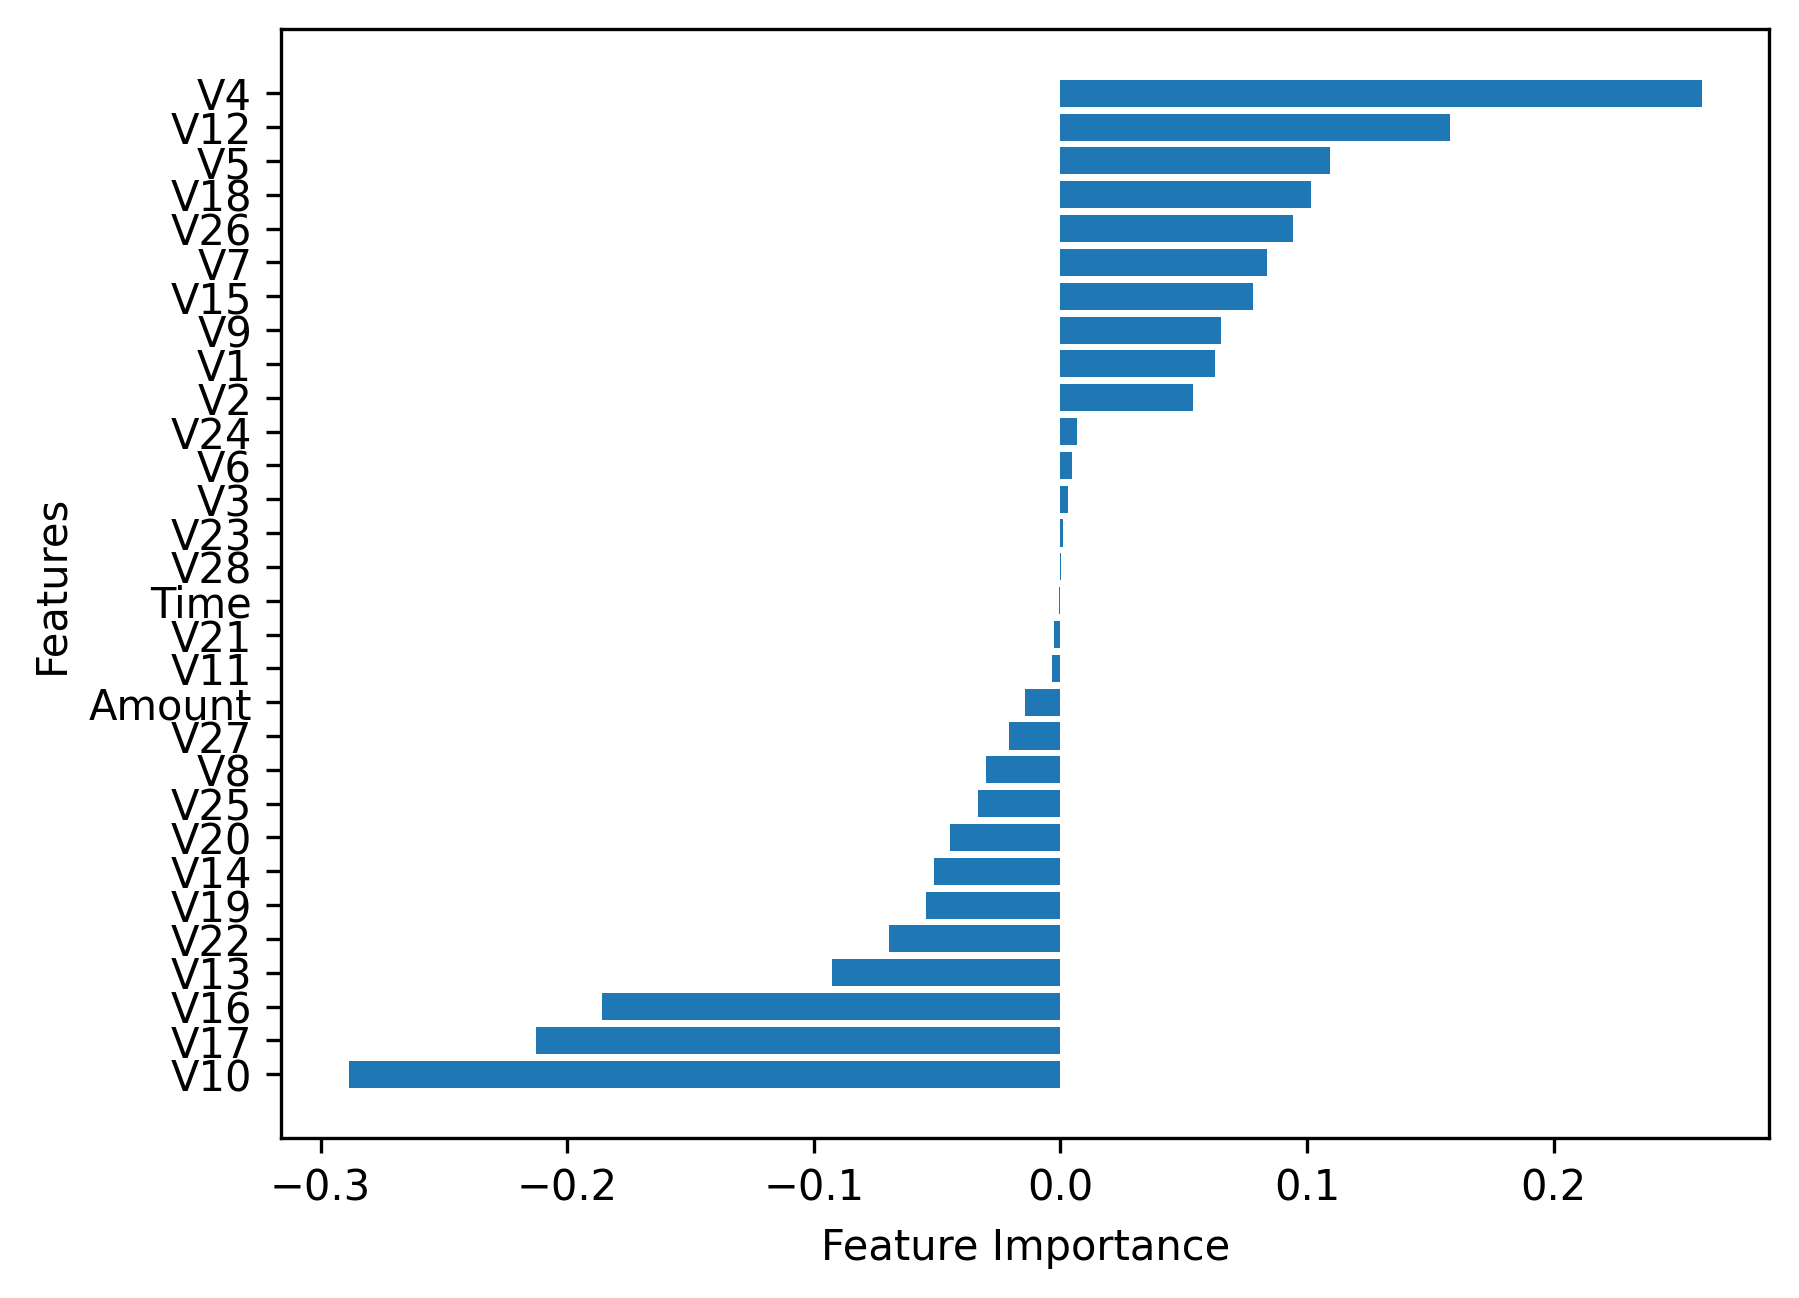
\includegraphics[width=\textwidth]{feature_importance.png}
\caption{Feature Importance}
\end{minipage}\hfill
\begin{minipage}{0.48\textwidth} 
Features V4, V12, and V5 strongly predict fraudulent transactions (Class 1), with higher values indicating genuine transactions. Conversely, V17, V16, and V10 are significant for real transactions, with lower values signaling fraud. 'Amount' and 'Time' have minor importance, implying they don't significantly aid class differentiation in the model.
\end{minipage}
\end{figure}

\begin{table}[H]
    \centering
    \caption{Classification Report}
    \label{tab:best_model_classification_report}
    \begin{tabular}{@{}lcccc@{}}
    \toprule
    Class & Precision & Recall & F1-Score & Support \\ \midrule
    0     & 1.00      & 1.00   & 1.00     & 56864   \\
    1     & 0.79      & 0.79   & 0.79     & 98      \\ \midrule
    Accuracy & \multicolumn{3}{c}{\hspace{3cm} 1.00} & \\ \midrule
    Macro Avg.  & 0.89      & 0.89   & 0.89     & 56962   \\
    Weighted Avg. & 1.00    & 1.00   & 1.00     & 56962   \\ \bottomrule
    \end{tabular}
\end{table}


The model's performance metrics reveal a precision of 1.00 for class 0 (genuine transactions) and 0.79 for class 1 (fraudulent transactions), indicating accurate positive predictions but a slight trade-off in identifying fraudulent transactions. The recall scores of 1.00 for class 0 and 0.79 for class 1 showcase the model's ability to correctly identify genuine transactions but with a similar trade-off in identifying fraudulent ones. The F1-scores, a balance of precision and recall, stand at 1.00 for class 0 and 0.79 for class 1, demonstrating strong performance overall with a consideration of trade-offs. With 56,864 instances of class 0 and 98 instances of class 1, the model's accuracy reaches 1.00, affirming its correctness in classifying instances. The macro-averaged metrics of precision, recall, and F1-score at 0.89 indicate good overall performance, while the weighted average F1-score of 1.00 underscores the model's excellent overall performance, particularly in handling imbalanced classes.


\begin{table}[H]
\centering
\caption{Confusion Matrix}
\begin{tabular}{|c|c|c|}
\hline
True\textbackslash Predicted & 0 & 1 \\
\hline
0 & 56843 & 21 \\
1 & 21 & 77 \\
\hline
\end{tabular}
\end{table}

The confusion matrix offers a granular view of a model's predictions, distinguishing between True Negatives (0,0), False Positives (0,1), False Negatives (1,0), and True Positives (1,1). In this case, there were 56,843 True Negatives, indicating instances correctly identified as genuine transactions. The model also had 21 False Positives, where transactions were inaccurately labeled as fraudulent when they were not. Conversely, there were 21 False Negatives, representing genuine transactions misclassified as fraudulent. Finally, the model accurately identified 77 instances as True Positives, correctly flagging them as fraudulent transactions. 


\section{Discussion}


\begin{figure}[H]
\centering
\begin{minipage}{0.48\textwidth} 
\centering
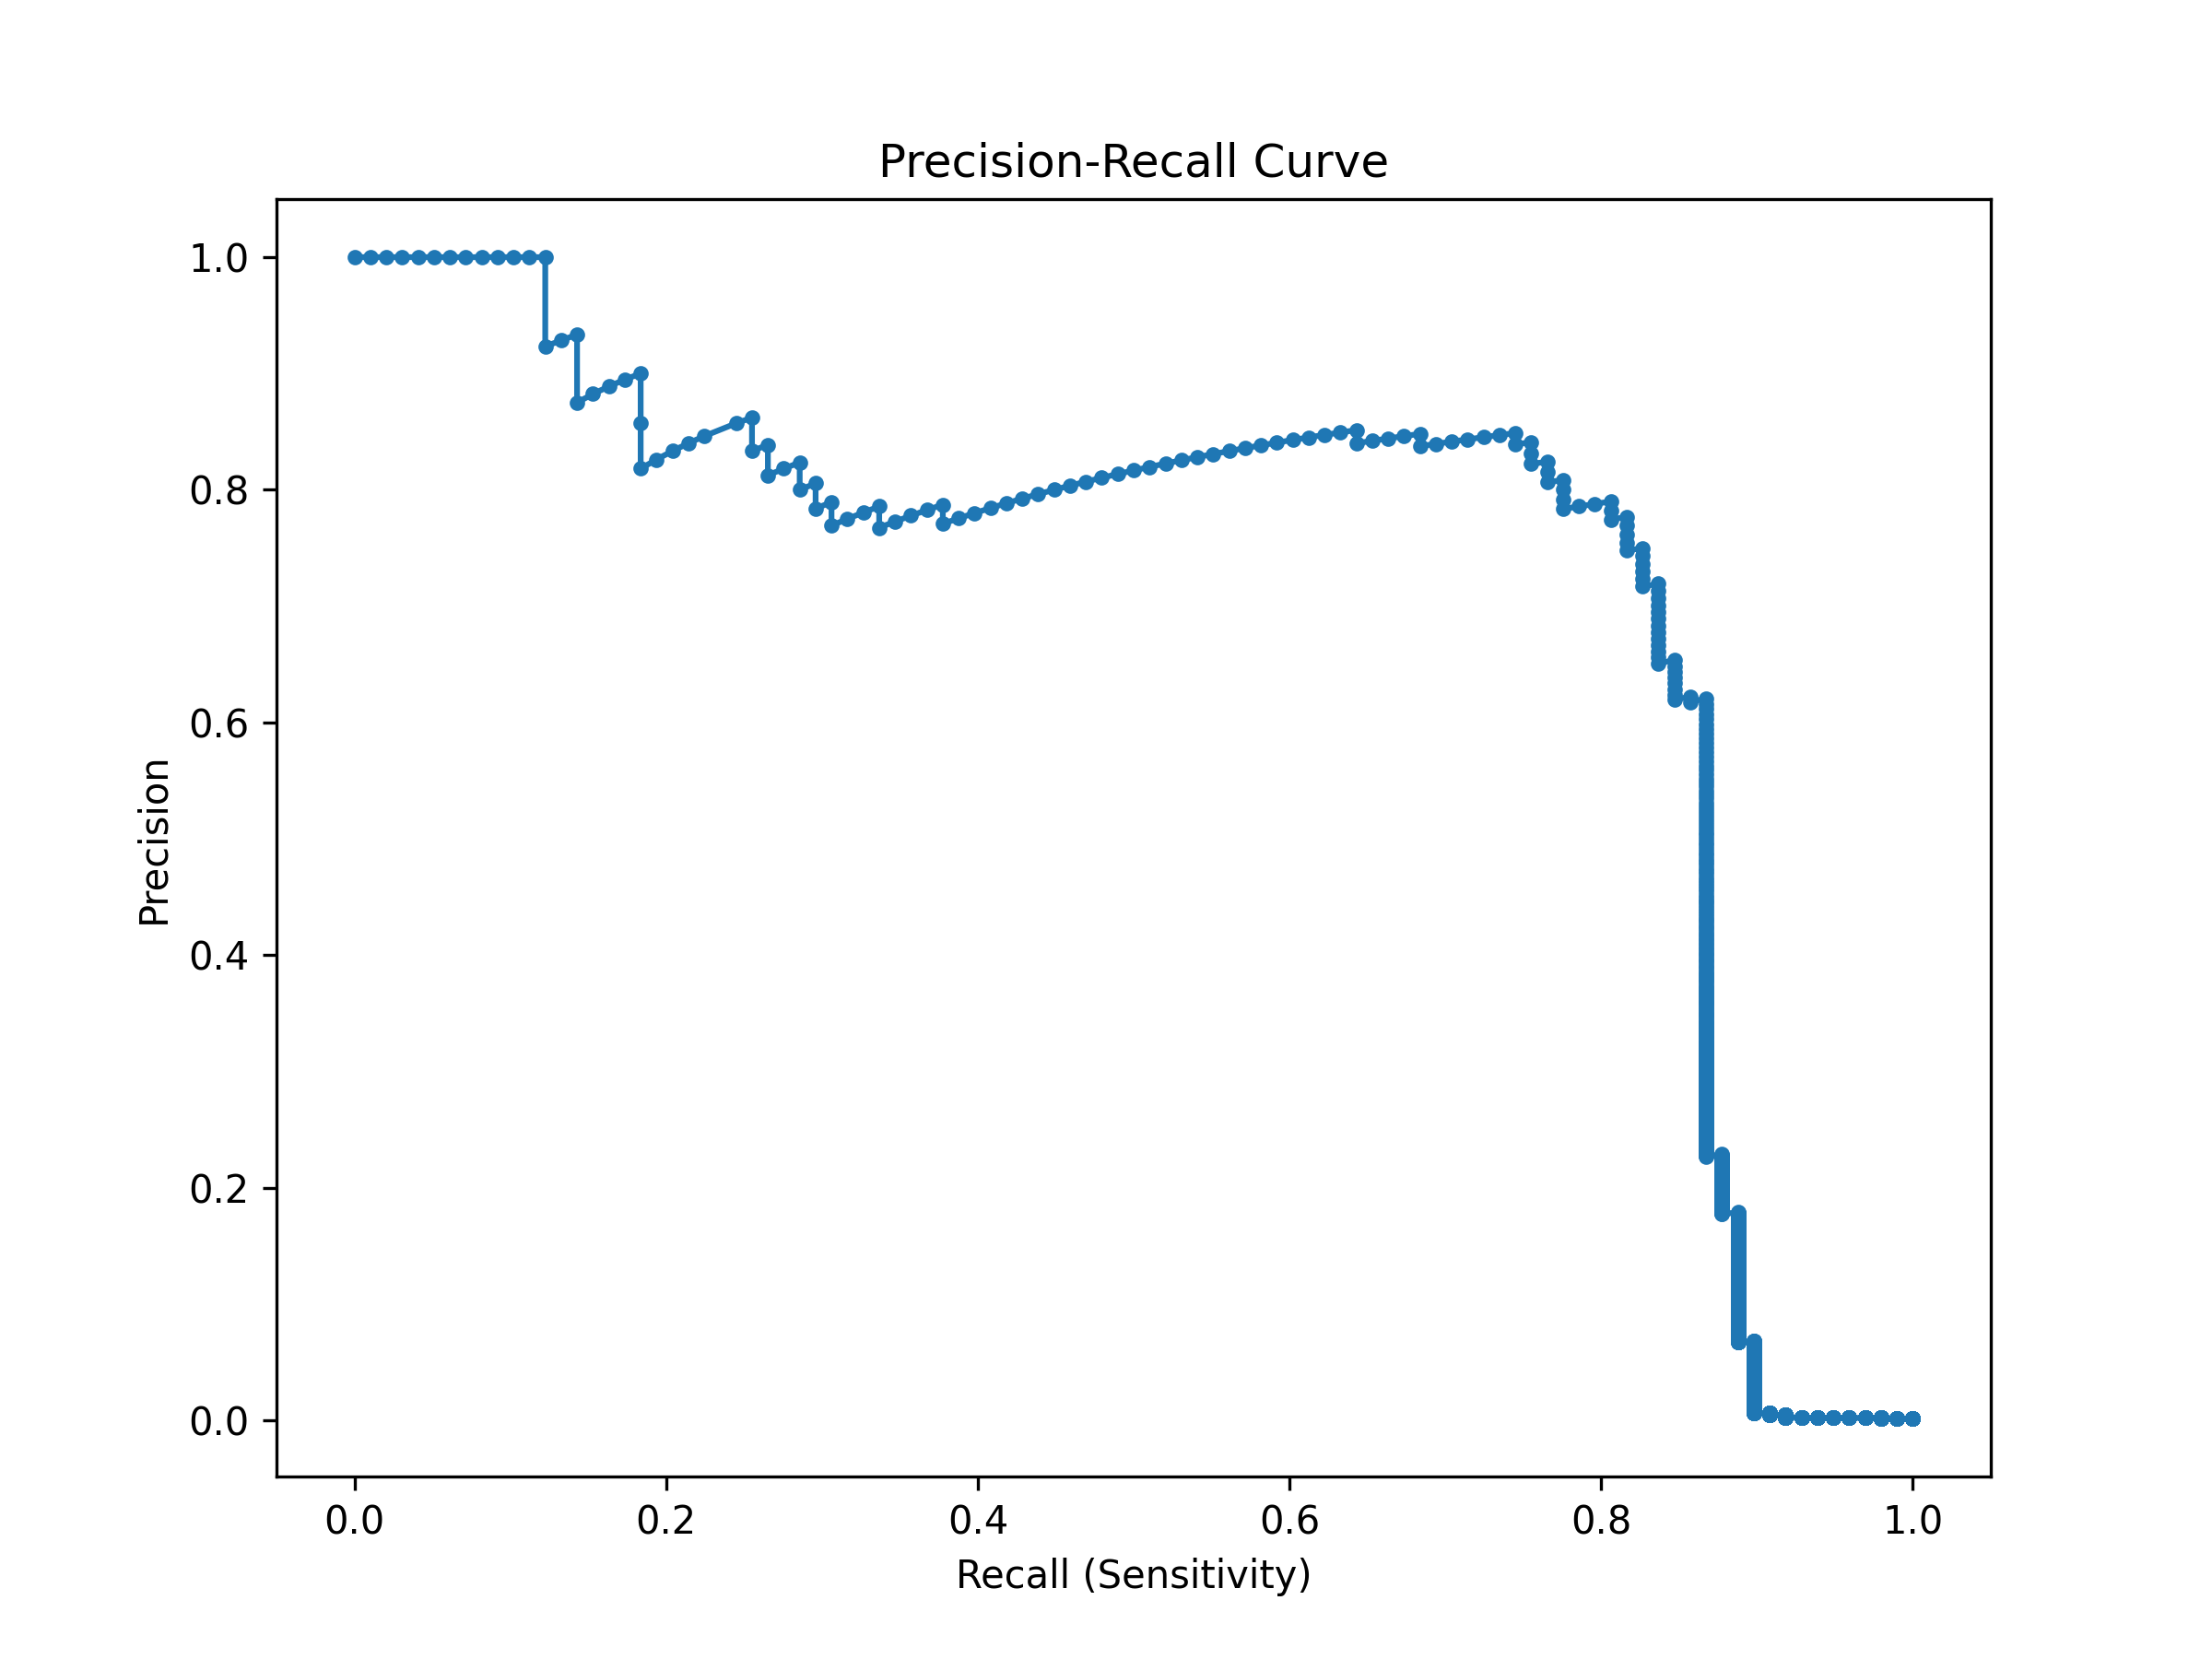
\includegraphics[width=\textwidth]{precision_recall_curve.png}
\caption{Feature Importance}
\end{minipage}\hfill
\begin{minipage}{0.48\textwidth} 
The precision-recall curve shows how the model's precision and recall change with different classification thresholds. Initially, high precision suggests accurate predictions but possibly misses some positives. As recall increases, precision decreases due to more false positives. The curve's steps indicate critical thresholds where small gains in recall lead to significant drops in precision, emphasizing the need for a balanced approach in fraud detection models.
\end{minipage}
\end{figure}

The results from the classification report and confusion matrix demonstrate the effectiveness of the model in fraud detection. The high precision of 1.00 for genuine transactions indicates that the model rarely misclassifies legitimate transactions as fraudulent. However, for fraudulent transactions, the precision of 0.79 suggests that approximately 79 of transactions flagged as fraudulent are indeed fraudulent. This trade-off between precision and recall in class 1 reflects the challenge of handling class imbalance. 

For class imbalance, various sampling techniques like SMOTE and class weights were used, but these approaches could not completely fix the problem. While these techniques offered a high recall score, they often led to a lower precision score. This discrepancy occurred because the synthetic samples generated by SMOTE and the adjusted class weights focused more on capturing minority class instances, thus increasing recall but sometimes at the expense of precision \cite{rnd1}. 

The recall of 1.00 for genuine transactions indicates that all actual legitimate transactions are correctly identified, while the recall of 0.79 for fraudulent transactions implies that the model captures about 79 percent of actual fraudulent transactions. The weighted average F1-score of 1.00 reflects the model's robustness and ability to handle class imbalance by considering the number of instances in each class. While the model demonstrates strong performance in classifying genuine transactions and reasonably good performance in identifying fraudulent transactions, there is room for further optimization. Strategies such as addressing class imbalance using advanced techniques like adversarial training could further enhance the model's effectiveness and reliability in real-world fraud detection scenarios, reducing financial losses and improving overall security in financial transactions \cite{rnd2}.

\printbibliography

\end{document}
